\documentclass[../../main.tex]{subfiles}
\begin{document}
\begin{oframed}
  \subfile{problem}
\end{oframed}

{\bf [解答]}

与えられた関数を
\begin{align}
  f(x)=\cos x+\dfrac{\sqrt{3}}{4}x^2 \quad \left(-\dfrac{\pi}{2} \le x \le \dfrac{\pi}{2}\right)
\end{align}
とおく．$f(x)$は偶関数だから以下$0\le x\le\pi/2$で調べれば良い．
$f'(x), f''(x)$を計算すると
\begin{align}
  & f'(x)=-\sin x +\dfrac{\sqrt{3}}{2}x \\
  & f''(x)=-\cos x + \dfrac{\sqrt{3}}{2}
\end{align}
だから，$f(x)$の増減表は以下のようになる．

\begin{table}[htb]
  \centering
  \caption{$f(x)$ の増減表（$0 \le x \le \pi/2$）}
  \label{tab:variation}
  \begin{tabular}{|c|c|c|c|c|c|c|c|}
    \hline
    $x$ & $0$ & $\cdots$ & $\pi/6$ & $\cdots$ & $\alpha$ & $\cdots$ & $\pi/2$ \\
    \hline
    $f''$ & & $-$ & $0$ & $+$ & $+$ & $+$ & \\
    \hline
    $f'$ & $0$ & $-$ & $\dfrac{-6+\sqrt{3}\pi}{12}$ & $-$ & $0$ & $+$ & $-1+\dfrac{\sqrt{3}}{4}\pi$ \\
    \hline
    $f$ & $1$ & $\searrow$ & $\dfrac{\sqrt{3}}{2}+\dfrac{\sqrt{3}\pi^2}{144}$ & $\searrow$ & 極小 & $\nearrow$ & $\dfrac{\sqrt{3}\pi^2}{16}$ \\
    \hline
  \end{tabular}
\end{table}

\begin{figure}[htb]
  \centering
  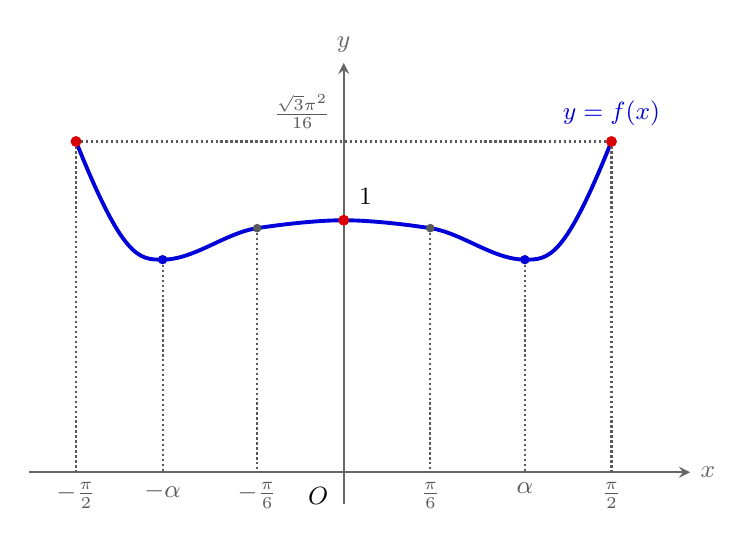
\begin{tikzpicture}[x=2.0cm, y=2.0cm, >=stealth,
    every node/.style={font=\small}]
    \coordinate (O) at (0,0);

    % Axes
    \draw[->, thick, gray!80!black] (-2.0,0) -- (2.2,0) node[right] {$x$};
    \draw[->, thick, gray!80!black] (0,-0.2) -- (0,2.6) node[above] {$y$};
    \node[below left=2pt] at (O) {$O$};

    % Graph of y = f(x) (schematic to clearly show the local minimum and inflection)
    % Coordinates: x = 0 -> y = 1.6, x = pi/6 (0.6) -> y = 1.5, x = alpha (1.15) -> y = 1.35, x = pi/2 (1.7) -> y = 2.1
    \draw[line width=1.4pt, blue!85!black]
    (-1.7, 2.1) .. controls (-1.4, 1.35) and (-1.3, 1.35) ..
    (-1.15, 1.35) .. controls (-0.95, 1.35) and (-0.75, 1.52) ..
    (-0.55, 1.55) .. controls (-0.35, 1.58) and (-0.15, 1.6) ..
    (0, 1.6) .. controls (0.15, 1.6) and (0.35, 1.58) ..
    (0.55, 1.55) .. controls (0.75, 1.52) and (0.95, 1.35) ..
    (1.15, 1.35) .. controls (1.3, 1.35) and (1.4, 1.35) ..
    (1.7, 2.1);

    % Characteristic points
    \coordinate (PmaxR) at (1.7, 2.1);
    \coordinate (PmaxL) at (-1.7, 2.1);
    \coordinate (P0) at (0, 1.6);
    \coordinate (PminR) at (1.15, 1.35);
    \coordinate (PminL) at (-1.15, 1.35);
    \coordinate (PinfR) at (0.55, 1.55);
    \coordinate (PinfL) at (-0.55, 1.55);

    % Dotted drop lines
    \draw[densely dotted, thick, gray!70!black] (PmaxR) -- (1.7,0) node[below] {$\frac{\pi}{2}$};
    \draw[densely dotted, thick, gray!70!black] (PmaxL) -- (-1.7,0) node[below] {$-\frac{\pi}{2}$};
    \draw[densely dotted, thick, gray!70!black] (-1.7,2.1) -- (1.7,2.1);
    \draw[densely dotted, thick, gray!70!black] (0,2.1) node[above left=1pt, font=\footnotesize] {$\frac{\sqrt{3}\pi^2}{16}$} -- (0,2.1);

    \draw[densely dotted, thick, gray!70!black] (PminR) -- (1.15,0) node[below] {$\alpha$};
    \draw[densely dotted, thick, gray!70!black] (PminL) -- (-1.15,0) node[below] {$-\alpha$};

    \draw[densely dotted, thick, gray!70!black] (PinfR) -- (0.55,0) node[below] {$\frac{\pi}{6}$};
    \draw[densely dotted, thick, gray!70!black] (PinfL) -- (-0.55,0) node[below] {$-\frac{\pi}{6}$};

    % Points
    \node[circle, fill=red!85!black, inner sep=1.4pt] at (PmaxR) {};
    \node[circle, fill=red!85!black, inner sep=1.4pt] at (PmaxL) {};
    \node[circle, fill=red!85!black, inner sep=1.4pt] at (P0) {};
    \node[circle, fill=blue!85!black, inner sep=1.2pt] at (PminR) {};
    \node[circle, fill=blue!85!black, inner sep=1.2pt] at (PminL) {};
    \node[circle, fill=gray!70!black, inner sep=1.1pt] at (PinfR) {};
    \node[circle, fill=gray!70!black, inner sep=1.1pt] at (PinfL) {};

    \node[above right=2pt] at (P0) {$1$};
    \node[blue!85!black, above=2pt] at (1.7,2.1) {$y=f(x)$};
  \end{tikzpicture}
  \caption{$y=f(x)$ の概形（$y$ 軸対称）}
  \label{fig:graph_f}
\end{figure}

ただし，
\begin{align}
  f'(\pi/2) = -1+\dfrac{\sqrt{3}}{4}\pi > 0 \\
  f'(\pi/6) = \dfrac{-6+\sqrt{3}\pi}{12} < 0
\end{align}
と$(\pi/6,\pi/2)$で$f''(x)>0$より$f'(x)$が単調増加であることから，この区間内に$f'(\alpha)=0$となる$\alpha$が存在する．

よって最大値の候補は，$f(0)=1$，$f(\pi/2)=\dfrac{\sqrt{3}\pi^2}{16}$であり，
\begin{align}
  f\left(\dfrac{\pi}{2}\right)>\dfrac{1.7\cdot(3.1)^2}{16}=\dfrac{16.337}{16}>1=f(0)
\end{align}
から，もとめる最大値は
\begin{align}
  \max f(x) =  f\left(\dfrac{\pi}{2}\right)=\dfrac{\sqrt{3}\pi^2}{16}
\end{align}
である．

\newpage

\end{document}
